%!TEX root = ../TAMUTemplate.tex
%%%%%%%%%%%%%%%%%%%%%%%%%%%%%%%%%%%%%%%%%%%%%%%%%%%
%
%  New template code for TAMU Theses and Dissertations starting Fall 2016.
%
%  Author: Sean Zachary Roberson
%	 Version 3.16.09
%  Last updated 9/12/2016
%
%%%%%%%%%%%%%%%%%%%%%%%%%%%%%%%%%%%%%%%%%%%%%%%%%%%

%%%%%%%%%%%%%%%%%%%%%%%%%%%%%%%%%%%%%%%%%%%%%%%%%%%%%%%%%%%%%%%%%%%%%%%
%%%                           SECTION II
%%%%%%%%%%%%%%%%%%%%%%%%%%%%%%%%%%%%%%%%%%%%%%%%%%%%%%%%%%%%%%%%%%%%%%


\chapter{\uppercase {The LHC and CMS Detector}}

\section{The Large Hadron Collider}

The Large Hadron Collider (LHC) \cite{Breskin:1244506} is, in many people's estimation, the largest and most complex machine ever built by humanity. The main accelerator at the European Organization for Nuclear Research (CERN), the LHC is located both in France and Switzerland due to its enormous size. It was built between 1998 and 2008 and installed in the $26.7\unit{km}$ tunnel dug for its predecessor, the Large Electron-Positron Collider (LEP), which is located between $50\unit{m}$ and $170\unit{m}$ underground. It is the highest energy collider in the world, eclipsing the previous record holder, the Tevatron at Fermilab in Batavia, IL. The following section is a description of the LHC and CERN accelerator complex based on \cite{LHCmachine} and \cite{Breskin:1244506}.

The LHC provides beams for four main experiments located along its beam line (Fig.~\ref{fig:LHC_schematic}):
\begin{itemize}
	\item The CMS (Compact Muon Solenoid)~\cite{Chatrchyan:2008aa} and ATLAS (A Toroidal LHC ApparatuS)~\cite{1748-0221-3-08-S08003} experiments are both general purpose detectors. Their goals include precision measurements to test the Standard Model and searches for new physics, including the Higgs boson.
	\item LHCb (Large Hadron Collider beauty)~\cite{Alves:2008zz} was designed to do precision measurements of CP-violation and the physics of B-mesons.
	\item ALICE (A Large Ion Collider Experiment)~\cite{Aamodt:2008zz} studies heavy ion collisions.
\end{itemize}

The LHC was designed to collide two beams of protons (pp), heavy ions (PbPb), or a combination of the two (pPb) at specific interaction points around the beam line. For the purposes of this thesis we will only cover proton-proton collisions from this point forward. The protons come from a single bottle of hydrogen gas, which is then disassociated and stripped of electrons to form a proton beam. Interestingly, only $1\unit{ng}$ of hydrogen is required per day in order to form the LHC beams. The protons next travel through the Linac2 machine where they form bunches and are accelerated to $50\unit{MeV}$. This chain continues through the Proton Synchroton Booster, the Proton Synchrotron, and the Super Proton Synchrotron where the protons are accelerated to $1.4\unit{GeV}$, $26\unit{GeV}$, and $450\unit{GeV}$ respectively. Finally the proton bunches are injected into the LHC beam pipes.




The design energy of the accelerator was $7\unit{TeV}$ with an instantaneous luminosity of up to $10^{34}\unit{cm^{-2}s^{-1}}$.









The following sections will only be concerned with the CMS experiment and the data it collected in 2012.

\begin{figure}[tb]
	\centering
	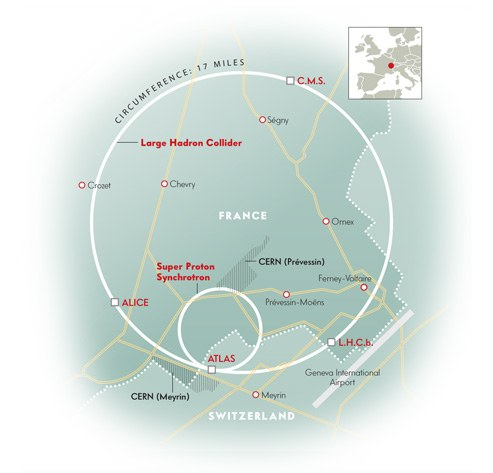
\includegraphics[width=0.95\textwidth]{\figpath/Chapter2/LHC_schematic.jpg}
	\caption{Overhead view of CERN and its main experiments, CMS; ATLAS; LHCb; and ALICE, as well as two of the larger accelerators, the LHC and SPS. The schematic is overlaid on a map of Switzerland and France~\cite{LHC-schematic}.}
	\label{fig:LHC_schematic}
\end{figure}

\begin{figure}[tb]
	\centering
	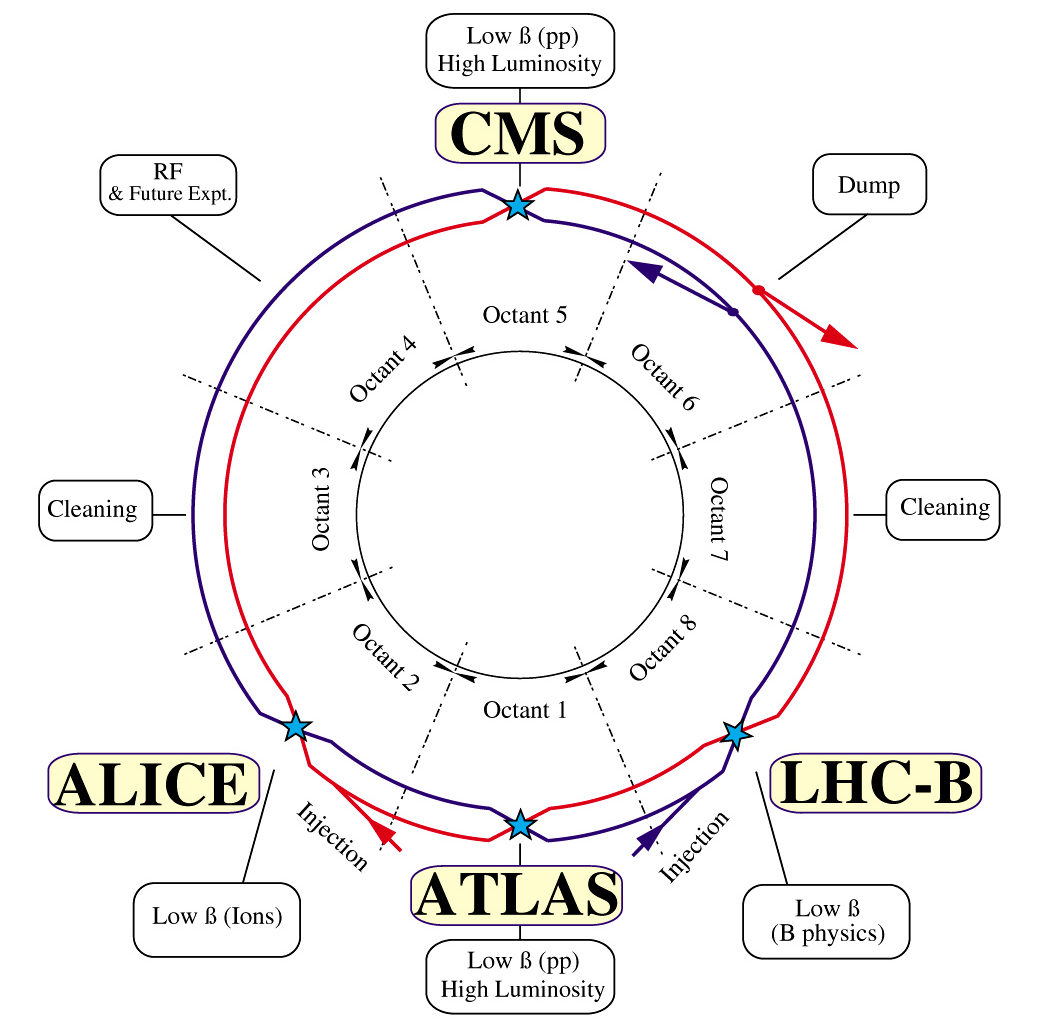
\includegraphics[width=0.95\textwidth]{\figpath/Chapter2/lhc-pho-1997-060.png}
	\caption{A diagram of the LHC beams along with the four major experiments~\cite{Jean-Luc:841573}.}
	\label{fig:LHC_beams}
\end{figure}

\begin{figure}[tb]
	\centering
	\begin{subfigure}[t]{0.4655\textwidth}
		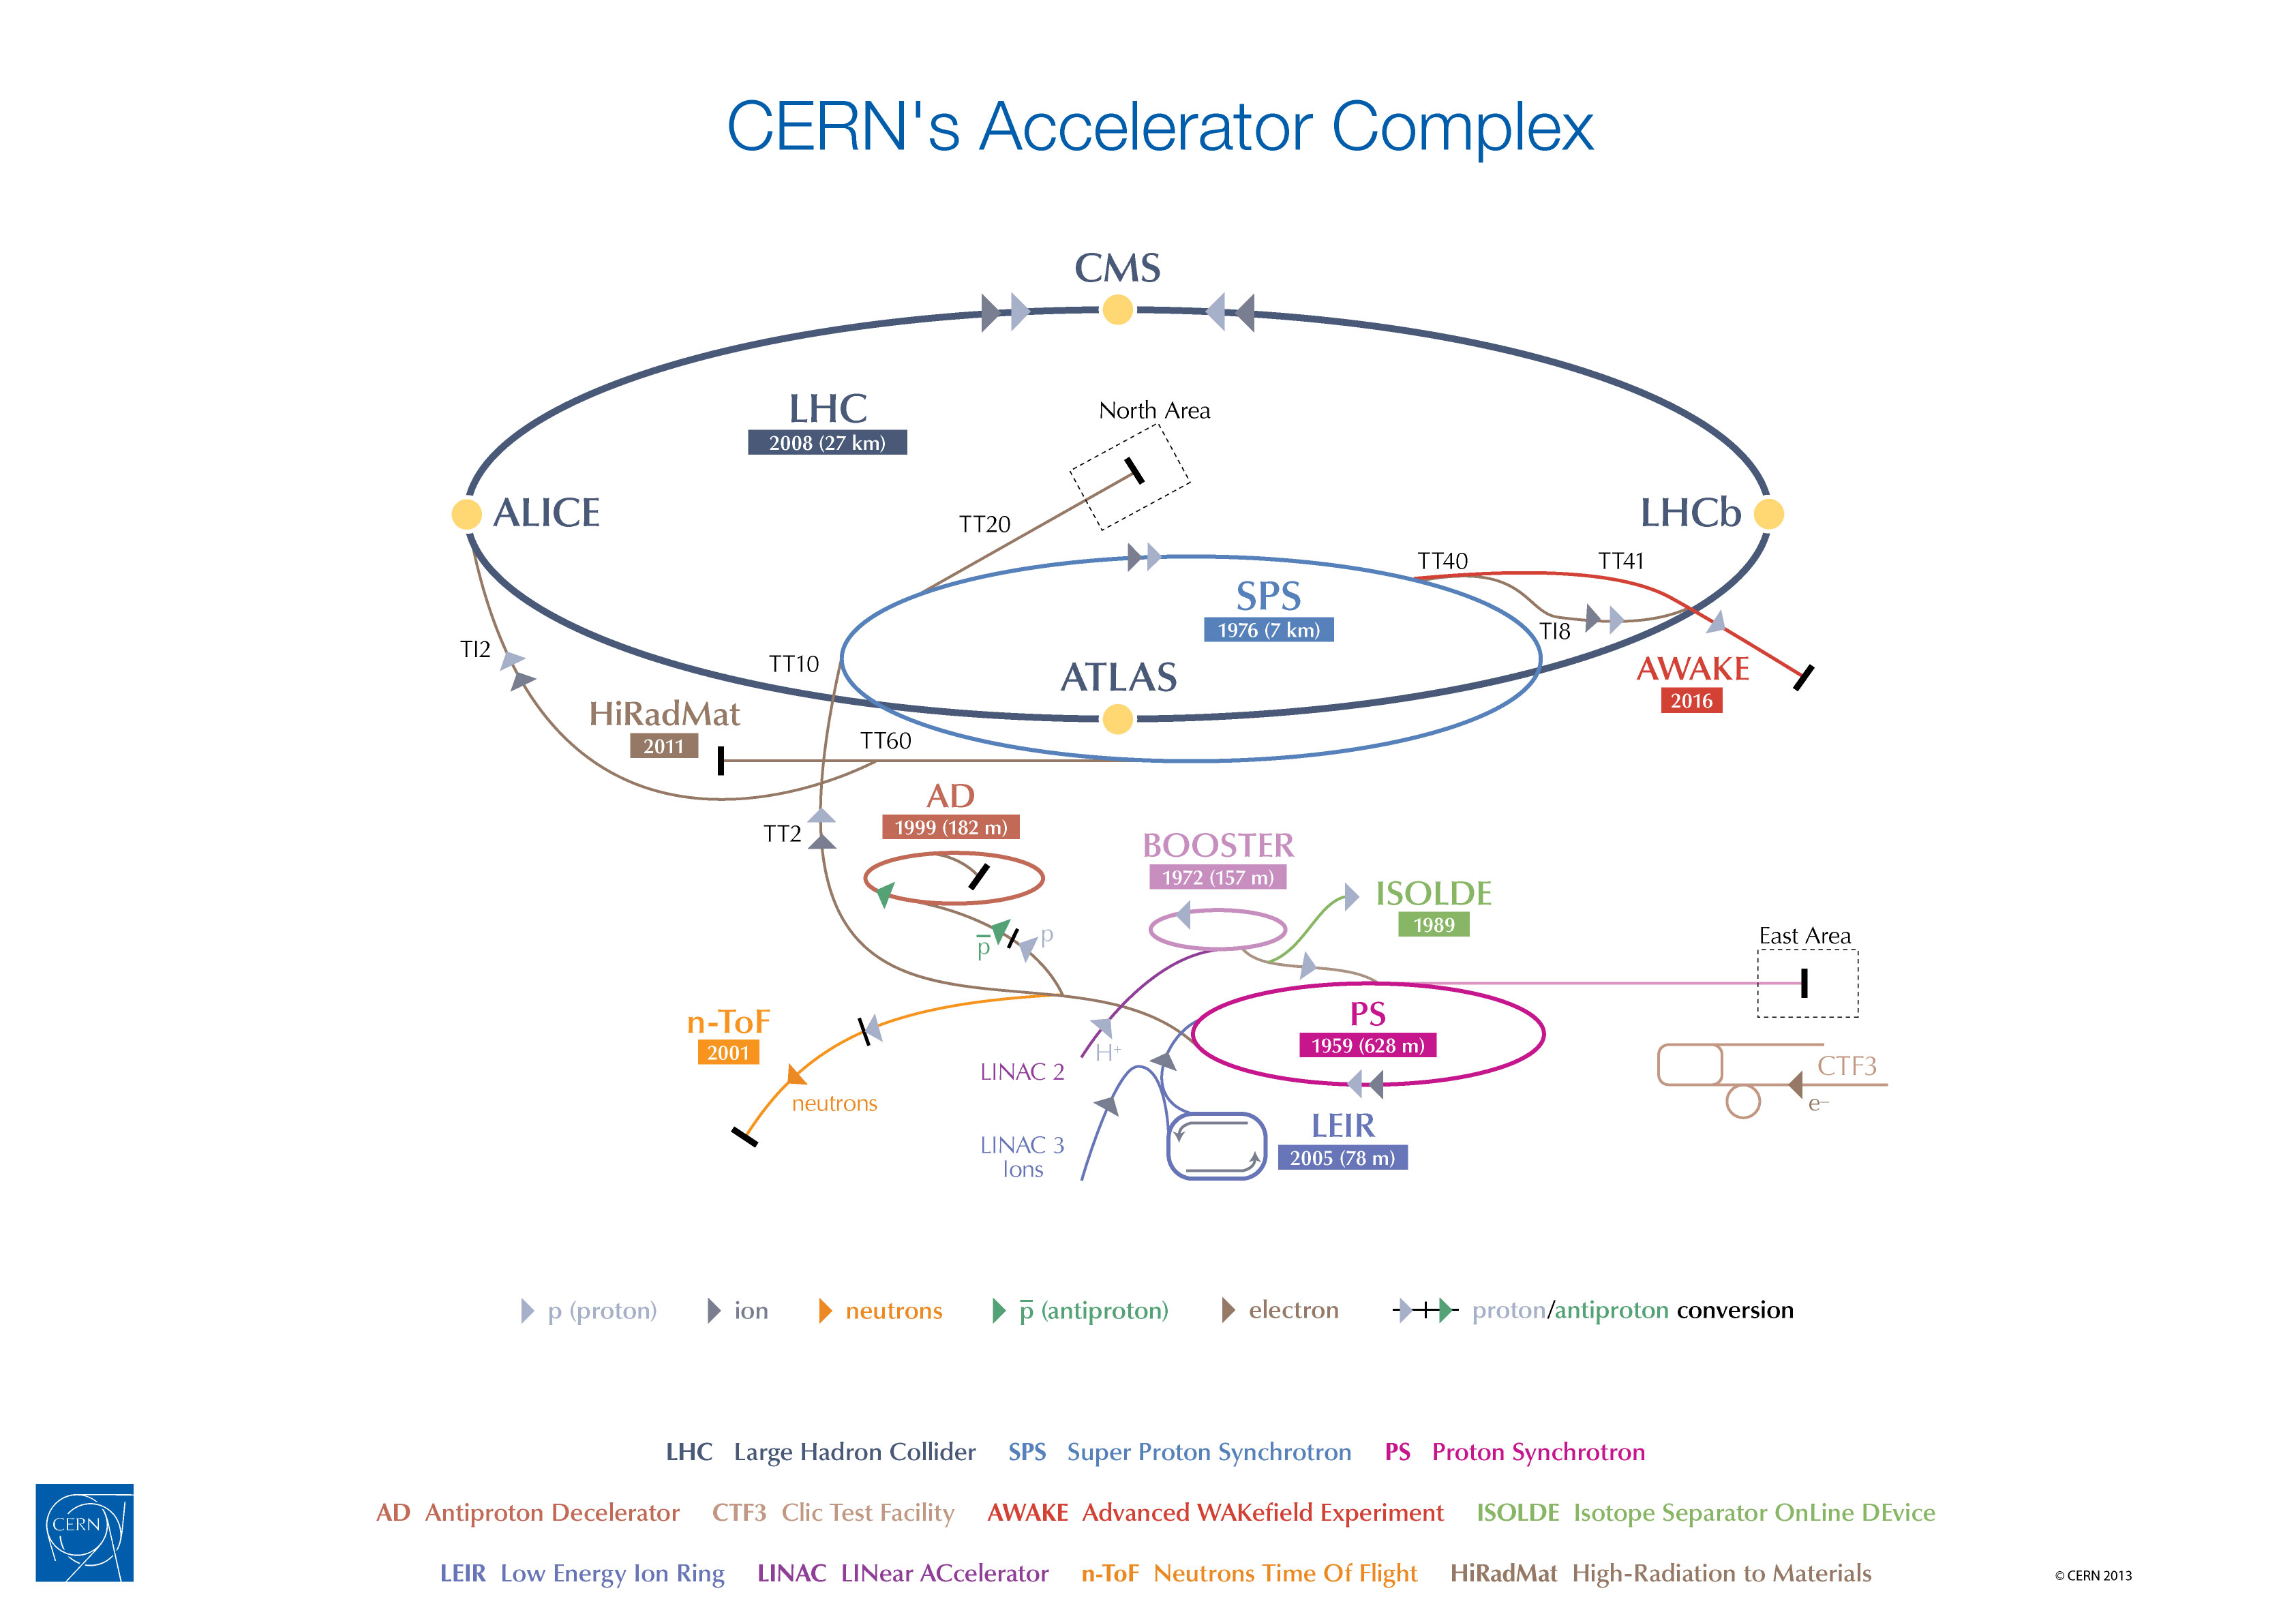
\includegraphics[width=\textwidth]{\figpath/Chapter2/CERN's-accelerator-complex2013.jpg}
		\caption{A schematic of the CERN accelerator complex~\cite{Marcastel:1621583}.}
		\label{fig:CERN_accelerator_complex}
	\end{subfigure}
	\begin{subfigure}[t]{0.4655\textwidth}
		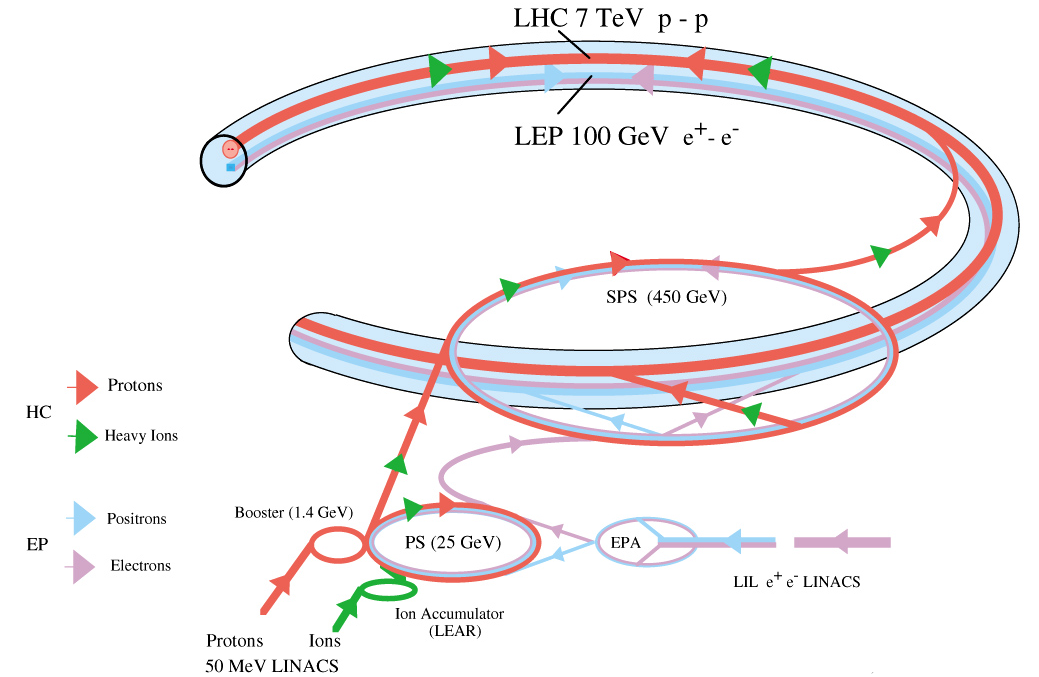
\includegraphics[width=\textwidth]{\figpath/Chapter2/lhc-pho-1993-008.png}
		\caption{A diagram of the LHC injection chain. Also included is a diagram of the heavy ion and LEP injection chains~\cite{Jean-Luc:841568}.}
		\label{fig:LHC_LEP_injection_complex}
	\end{subfigure}
\end{figure}

\begin{figure}[tb]
	\centering
	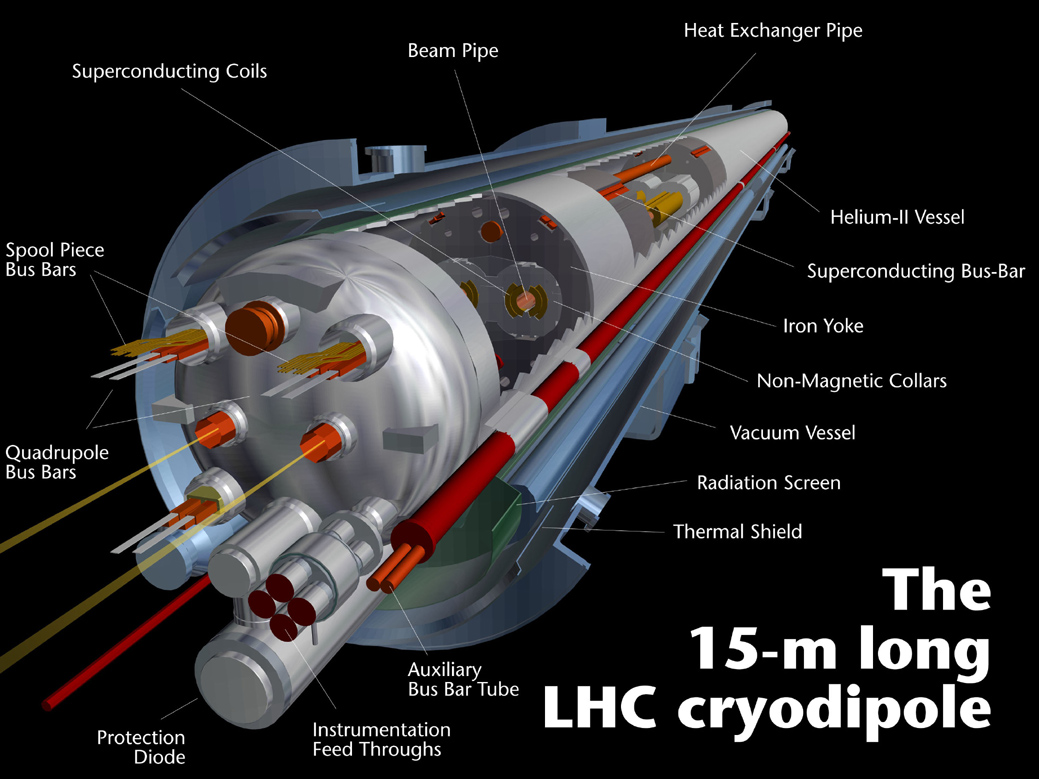
\includegraphics[width=0.95\textwidth]{\figpath/Chapter2/lhc-pho-1998-299.jpg}
	\caption{A diagram of an LHC dipole magnet and cryostat~\cite{Dailler:842253}.}
	\label{fig:CERN_accelerator_complex}
\end{figure}


\section{The CMS Detector}
\subsection{Coordinate System}
\subsection{Tracker and Pixel Detector}
\subsection{Electromagnetic Calorimeter}
\subsection{Hadron Calorimeter}
\subsection{Solenoid}
\subsection{Muon System}
\subsection{Trigger}
\subsection{Luminosity Measurement}